\documentclass{article}

\usepackage[]{graphicx}
\usepackage[]{float}

\title{
	Canning for Amorphous Blob Computing\\
	\small TER report
}

\author{
    Auteur :\\
    Lucas Labouret\\
    M1 QDCS, Université Paris-Saclay\\
    \small lucas.labouret@universite-paris-saclay.fr
    \and
    Encadrant :\\
    Frédéric Gruau\\
    LISN\\
    \small frederic.gruau@universite-paris-saclay.fr
}

\date{}

\begin{document}
 
\maketitle

\begin{figure}[H]
	\centering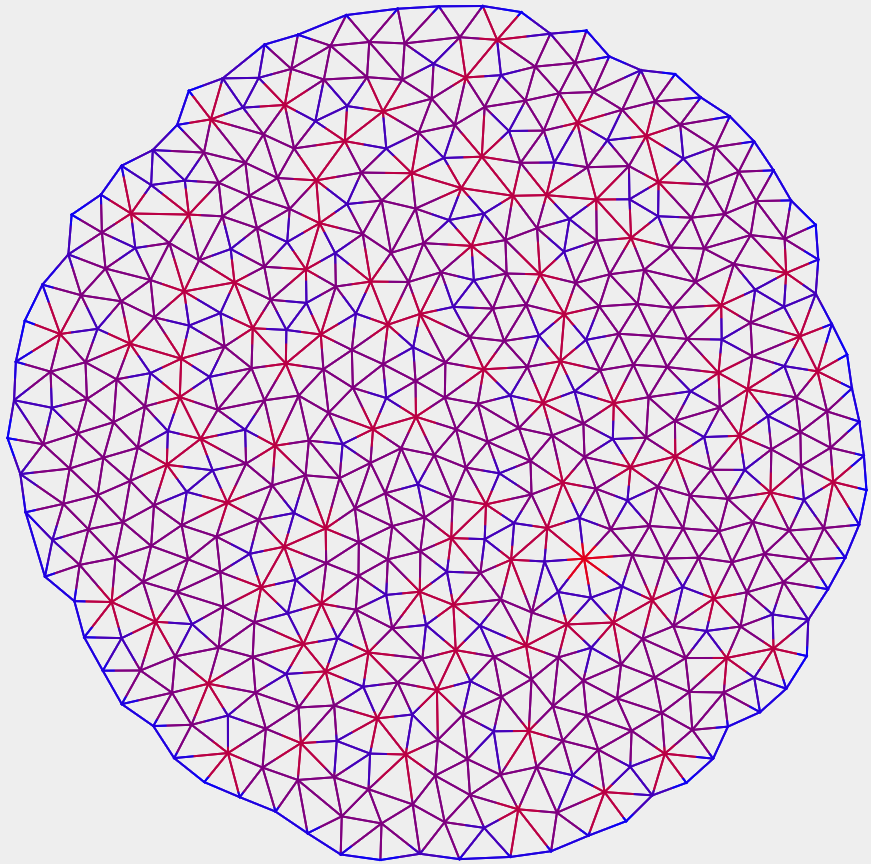
\includegraphics[width=0.9\linewidth]{assets/Circle500.png}
\end{figure}

\newpage
\tableofcontents
\newpage

\renewcommand{\thesection}{\Alph{section}}

\section{What is blob computing ?}

\subsection{Computing media}

\subsection{An example of computation : the Voronoï diagram}

\subsection{Objective : Cannings}

\section{Preliminary work}

\subsection{Delaunay Triangulation}

\subsection{Furthest Point Optimization}


\renewcommand{\thesection}{\arabic{section}}
\setcounter{section}{0}

\section{GUI}

\section{Borders and media}

\subsection{Choice of border}

\subsection{Different types of medium}

\section{Canning and evaluation}

\subsection{Partial and total cannings}

\subsection{Evaluation}

\end{document}
